\documentclass[10pt,a4paper]{article}
\usepackage[utf8]{inputenc}
\usepackage{amsmath}
\usepackage{amsfonts}
\usepackage{amssymb}
\usepackage{graphicx}
\usepackage{times}
\usepackage{verbatim}
\usepackage{listings} 
\usepackage{graphicx}
\author{Mashruf Zaman Chowdhury}
\pagestyle{plain}
\usepackage[top=1in, bottom=1in, left=1.5in, right=1.5in]{geometry}


\usepackage{enumitem}
\setitemize{nolistsep,leftmargin=*}


\usepackage{listings}
\usepackage{color}

\definecolor{dkgreen}{rgb}{0,0.6,0}
\definecolor{gray}{rgb}{0.5,0.5,0.5}
\definecolor{mauve}{rgb}{0.58,0,0.82}

\lstset{frameround=ffff,
  language=bash,
  aboveskip=2mm,
  belowskip=2mm,
  showstringspaces=false,
  columns=flexible,
  basicstyle={\small\ttfamily},
  numbers=none,
  numberstyle=\tiny\color{blue},
  keywordstyle=\color{blue},
  commentstyle=\color{dkgreen},
  stringstyle=\color{blue},
  breaklines=true,
  breakatwhitespace=true,
  tabsize=3
}

\begin{document}
\title{Robotics Project: ROS-Turtlebot Motion Control $\&$ Navigation} \author{Yanik Porto \and Mashruf Zaman \and AK Assad} \date{\today}
\maketitle

\lstset{language=Python}% Set your language (you can change the language for each code-block optionally)

\tableofcontents

\newpage
\section[Part 1 - Motion Control]{Part 1 - Motion Control}

\subsection{Understanding the basics}

\begin{itemize}
\itemsep0em 
\item Nodes: A node is an executable that uses ROS to communicate with other nodes.
\item Messages: ROS data type used when subscribing or publishing to a topic.
\item Topics: Nodes can publish messages to a topic as well as subscribe to a topic to receive messages.
\item Master: Name service for ROS (i.e. helps nodes find each other)
\item rosout: ROS equivalent of stdout/stderr, This is always running as it collects and logs nodes' debugging output.
\item roscore: Master + rosout + parameter server %
(parameter server will be introduced later)
\end{itemize}

\subsection{Levels of Motion Control}
Controlling a mobile robot can be done at a number of levels and ROS provides methods for most of them.

\begin{center}
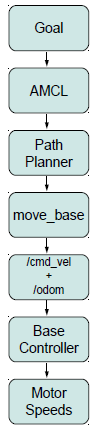
\includegraphics[width=0.2\textwidth]{motion_control.png}\\
\end{center}

\subsubsection{Motors, Wheels and Encoders}
Turtlebot uses \textbf{Encoders} to drive it's motors or wheels. Encoder registers certain number of ticks per revolution for a wheel. Knowing the diameter and distance between the wheels, from these ticks we can find distance traveled by the robot. To compute speed, these values are simply divided by the time interval between measurements.
This internal motion data is known as \fbox{odometry}. Due to Environmental and other errors this data is not generally accurate. We need to use other motion data sources to get better estimation.

\subsubsection{Motor Controllers and Drivers}
At the lowest level of motion control, a \textbf{driver }for the robot's motor controller turns the wheels at a desired speed, usually using internal units such as \textbf{encoder ticks per second} or a percentage of max speed.

\subsubsection{The ROS Base Controller}
At this level of abstraction, the desired speed of the robot is specified in real-world units such as meters and radians per second. It also commonly employs some \textbf{PID control }(Proportional Integral Derivative), which in layman terms generally does it's best to move the robot in the way we have requested. 

The driver and PID control are combined inside a single ROS node called \textbf{base controller}. 

The base controller node typically publishes odometry data on the \textbf{/odom }topic and listens for motion commands on the \textbf{/cmd\_vel} topic.

Also a transform from the \textbf{/odom} frame to the base frame—either \textbf{/base\_link} or /\textbf{base\_footprint (Turtlebot)} is done depending on the robot types.

Once we have our \textbf{base controller with a ROS interface} our programming can focus purely on the desired linear and angular velocities in real-world units.

\subsubsection{Frame-Base Motion using the move\_base ROS Package}
The \textbf{move\_base} package is a very sophisticated path planner and combines \textbf{odometry data} with both \textbf{local and global cost maps }when selecting a path for the robot to follow. We discuss more about \textbf{move\_base} in Navigating with Path Planning section.

\subsubsection{SLAM using the gmapping and amcl ROS Packages}
At an even higher level, ROS enables our robot to create a map of its environment using the SLAM gmapping package.

Once a map of the environment is available, ROS provides the amcl package (adaptive Monte Carlo localization) for automatically localizing the robot based on its current scan and odometry data.

\subsubsection{Semantic Goals}
Finally, at the highest level of abstraction, motion goals are specified semantically such as "go to the kitchen and bring me a beer", or simply, "bring me a beer". These are generally segmented into smaller tasks and passed to lower levels.

\subsection{Setting up the Network}

The primary requirement for getting your TurtleBot running is connecting to a network so that we can operate it remotely. After both TurtleBot and Workstation is connected to a network, it is time to set ROS\_MASTER\_URI and ROS\_HOSTNAME. The ROS\_MASTER\_URI tells the rest of the nodes at which address they can find the ROS master.\\

Here we setup the TurtleBot netbook as a ROS node and our Workstation as a ROS master. Before this is done, we need to determine the IP address of your TurtleBot netbook and Workstation. This can be found by typing ``ifconfig'' in a terminal. Our IP address are found under wlan0, and it's the numbers proceeding ``inet addr:''.

\begin{lstlisting}[frame=single] 
> echo export ROS_MASTER_URI=http://IP_OF_WORKSTATION:11311 >> ~/.bashrc
> echo export ROS_HOSTNAME=IP_OF_TURTLEBOT >> ~/.bashrc
\end{lstlisting}
For ROS to operate you need to have an instance of roscore running on the master. We type the following command in the master:

\begin{lstlisting}[frame=single] 
$ roscore
\end{lstlisting}
These commands will add the export lines to the system bashrc file so they will run on every new terminal instance. This could also be done using an editor with command like $gedit \sim/.bashrc$ and saving the IP addresses there.

\subsection{Testing with the fake and the real Turtlebot}
The programs can be tested both in a simulated environment and in the real robot. However, when testing the real robot using the current configuration of the kobuki base in the turtlebot, it is necessary to remap the topic $\textbf{/mobile\_base/commands/velocity}$ to $/\textbf{cmd\_vel}$. In order do this, a launch file is created to remap this topic, in fact in every launch file we changed the topic like this.

\subsection{Testing a node - Turtlebot Follower}
We initiate the turtlebot from our workstation:
\begin{lstlisting}[frame=single]
$ ssh turtlebot@192.168.0.100 , Password:napelturbot
$ roslaunch turtlebot_le2i remap_rplidar_minimal.launch (Bring up turtlebot)
$ roslaunch turtlebot_follower follower.launch (Start follower demo)
\end{lstlisting}
Now the Turtlebot detects and follows the person/obstacle in front of it.
[link of the video]

\subsection{Testing a node - Auto Docking}
We launch the kobuki core by typing:

\begin{lstlisting}[frame=single] 
$ roslaunch kobuki_auto_docking compact.launch --screen
\end{lstlisting}
But it is just loading the algorithm, which is still not active. The algorithm is implemented as a typical action server. We need to call the server via an action client:

\begin{lstlisting}[frame=single] 
$ roslaunch kobuki_auto_docking activate.launch --screen
\end{lstlisting}

But for our case it did find the dock perfectly but with a slight error.
[link of the video]


\subsection{Goal 1 Basic Motion of Mobile Base}

We can do this in two way - from command prompt or by using a node. We see both way - 
\subsubsection{From command prompt}
ROS uses the \textbf{Twist message} type for publishing motion commands to be used by the base controller. While we could use almost any name for a topic, it is usually called \textbf{/cmd\_vel} which is short for "command velocities". The base controller node subscribes to the \textbf{/cmd\_vel} topic and translates \textbf{Twist messages} into motor signals that actually turn the wheels.

We can see the components of a \textbf{Twist message} using the following command:\\\\
\fbox{\$rosmsg show geometry\_msgs/Twist}\\

The Twist message is composed of two sub-messages with type Vector3, one for the x, y and z linear velocity components and another for the x, y and z angular velocity components. Linear velocities are specified in \underline{meters per second} and angular velocities are given in \underline{radians per second}.\\

By the following command we say the robot to go in linear direction 0.15 meter/s and at the same time change angular direction (z axis) clockwise 0.4 rad/s. For example if we wanted to rotate a full revolution per 2 second we had to use 3.14 as z value.
\begin{lstlisting}[frame=single] 
$roslaunch turtlebot_le2i remap_rplidar_minimal.launch (Bring up turtlebot)
$rostopic pub -r 10 /cmd_vel geometry_msgs/Twist '{linear: {x: 0.15, y: 0, z: 0}, angular: {x: 0, y: 0, z: -0.4}}'
\end{lstlisting}
We initialize the launch file and Publish \textbf{geometry\_msgs/Twist} message in the \textbf{/cmd\_vel} topic using ``rostopic'' command. Here \textbf{-r} is an option by which we say to do 10 repetitions.

\subsubsection{By using a node}
To do this we run a python script from ROS-by-Example (rbx1) packages. At first we go to our \textbf{/ros\_workspace} directory and clone the repo and make the package using the following commands:

\begin{lstlisting}[frame=single] 
$git clone https://github.com/pirobot/rbx1.git
$cd rbx1
$rosmake
$rospack profile
\end{lstlisting}

From command prompt we just use one command at a time. But we want to do some sequential tasks, so it is better to give commands again and again then to put them in a source code file or node. \\
We use timed Twist commands to move the robot forward a certain distance, rotate 180 degrees, then move forward again for the same time and at the same speed where it will hopefully end up where it started. Finally, we will rotate the robot 180 degrees one more time to match the original orientation.\\\\

This is a \textbf{Time and Speed} based approximation, which we shall see will not be as accurate as expected. Here are the code segments to do it:

We ssh into the turtlebot and run the follwing scripts
on Turtlebot:
\begin{lstlisting}[frame=single] 
$roslaunch turtlebot_le2i remap_rplidar_minimal.launch (Bring up turtlebot)
\end{lstlisting}
We are going to configure to subscribe to combined odometry data (encoders + gyro) 
rather than \textbf{/odom} topic which only shows the encoder data. Hence we run this script
\begin{lstlisting}[frame=single] 
$roslaunch rbx1_bringup odom_ekf.launch
\end{lstlisting}

\textbf{On Workstation:}\\
run \textbf{rviz} to see the combined odometry data. This is displaying the combined odometry data on the \textbf{/odom\_ekf} topic rather than just the wheel encoder data published on the \textbf{/odom} topic.
\begin{lstlisting}[frame=single] 
$rosrun rviz rviz -d `rospack find rbx1_nav`/nav_ekf.rviz
\end{lstlisting}
finally we run the python script to do the previously defined task 
\begin{lstlisting}[frame=single] 
$rosrun rbx1_nav timed_out_and_back.py
\end{lstlisting}

Now we can see from rviz is that, the robot didn't do actually what is supposed to do
because of environmental constraint. It messed up but we have unfairly handicapped it 
by not using the odometry data in our script. Our script based only on time and speed. 
While the odometry data will not match the real motion exactly, 
it should give us a better result if we use it. We shall see it in the next step

\subsection{Goal 2 = Advanced Motion of Mobile Base}
let's assume that we have some data from the laser in the form of distances from the laser's center point. In other words, we have some data in the \textbf{``base\_laser"} coordinate frame. Now suppose we want to take this data and use it to help the mobile base avoid obstacles in the world. To do this successfully, we need a way of transforming the laser scan we've received from the \textbf{``base\_laser"} frame to the \textbf{``base\_link"} frame. In essence, we need to define a relationship between the \textbf{``base\_laser"} and \textbf{``base\_link"} coordinate frames.\\

\begin{center}
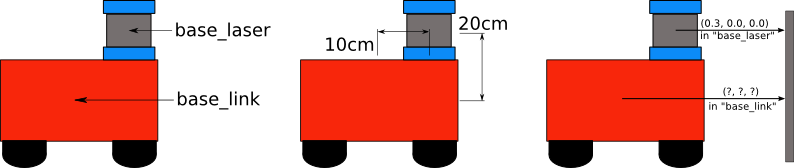
\includegraphics[width=\textwidth]{simple_robot.png}\\
\end{center}

Such is the case for the turtlebot Odometry data we use to move the robot.
While the \textbf{/base\_link} frame corresponds to a real physical part of Controlling a Mobile Base robot, the \textbf{/odom} frame is defined by the translations and rotations encapsulated in the odometry data. These transformations move the robot relative to the \textbf{/odom} frame.
In ROS if we see the \textbf{nav\_msgs/Odometry} message structure, \textbf{/odom }is used as the parent frame and \textbf{/base\_footprint} (for turtlebot) as the \textbf{child\_frame\_id}. The transformation between these two frames, is with the help of tf library.\\

Rather than guessing distances and angles based on time and speed, our next script will monitor the robot's position and orientation as reported by the transformation between the \textbf{/odom }and \textbf{/base\_footprint} frames.\\
 

We ssh into the turtlebot and run the follwing scripts
on Turtlebot:
\begin{lstlisting}[frame=single] 
$roslaunch turtlebot_le2i remap_rplidar_minimal.launch (Bring up turtlebot)
\end{lstlisting}
We are going to configure to subscribe to combined odometry data (encoders + gyro) 
rather than \textbf{/odom }topic which only shows the encoder data. Hence we run this script
\begin{lstlisting}[frame=single] 
$roslaunch rbx1_bringup odom_ekf.launch
\end{lstlisting}

On Workstation:
run rviz to see the combined odometry data
This is displaying the combined odometry data on the \textbf{/odom\_ekf} 
topic rather than just the wheel encoder data published on the \textbf{/odom} topic.
\begin{lstlisting}[frame=single] 
$rosrun rviz rviz -d `rospack find rbx1_nav`/nav_ekf.rviz
\end{lstlisting}

finally we run the python script to do the previously defined task 
\begin{lstlisting}[frame=single] 
$rosrun rbx1_nav odom_out_and_back.py
\end{lstlisting}

Using odometry the results improves significantly from the timed out-and-back case, because still accuracy and reliability of this process depends on the robot's internal sensors, the accuracy of the calibration procedure, and environmental conditions.
Since the robot is performing a very simple task, the navigation error is slight, and it is more evident after performing the task successively several times.

\subsubsection{Dead Reckoning}
Even small amount of error in the robot odometry data accumulates over time. Hence a robot navigating only using internal motion data and without any reference to external landmarks will grow on it's mistakes and eventually be completely lost. This is knows as Dead Reckoning. \\
We can improve this for our turtlebot using map and SLAM.

\subsection{Goal 3 = Navigating a Square using Twist+Odometry}
In a similar way to the previous Goal, in Goal 3 the robot navigates through a square path, using both Twist and Odometry messages.

However, this time we will attempt to move the robot in a square by setting four waypoints, one at each corner. At the end of the run, we can see that the errors accumulated in odometry are more visible:


\subsection{Goal 4 = Navigation with Path Planning move\_base}
ROS provides the move\_base package that allows us to specify a target position and orientation of the robot with respect to some frame of reference.

Following figure summarizes how the move\_base path planner works. On the bottom left of figure is a base controller node for low level motion control. on the top right is the map server which provides a map of environment.

\begin{center}
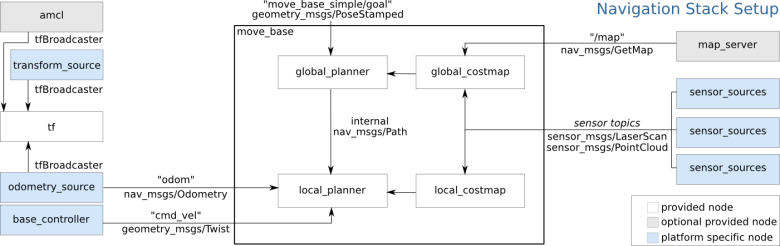
\includegraphics[width=\textwidth]{overview_small.png}
\end{center}
\section{Part 2 - Planar Laser RangeFinder}


\section{Part 3 - Navigation $\&$ Localization}

\section{Part 4 - Controlling with Android}


something

\end{document}